\begin{frame}{Anticipatory Reasoning in multi-agent simulations}
\begin{columns}
\visible<1->{
\begin{column}{.5\linewidth}
\vspace{.3cm}
\begin{figure}
    
\includegraphics[width=\linewidth]{figures/classic_anticipation.png}
    \caption{Classical anticipatory reasoning}
\end{figure}

\end{column}
}
\visible<2->{
\begin{column}{.5\linewidth}
\begin{figure}
    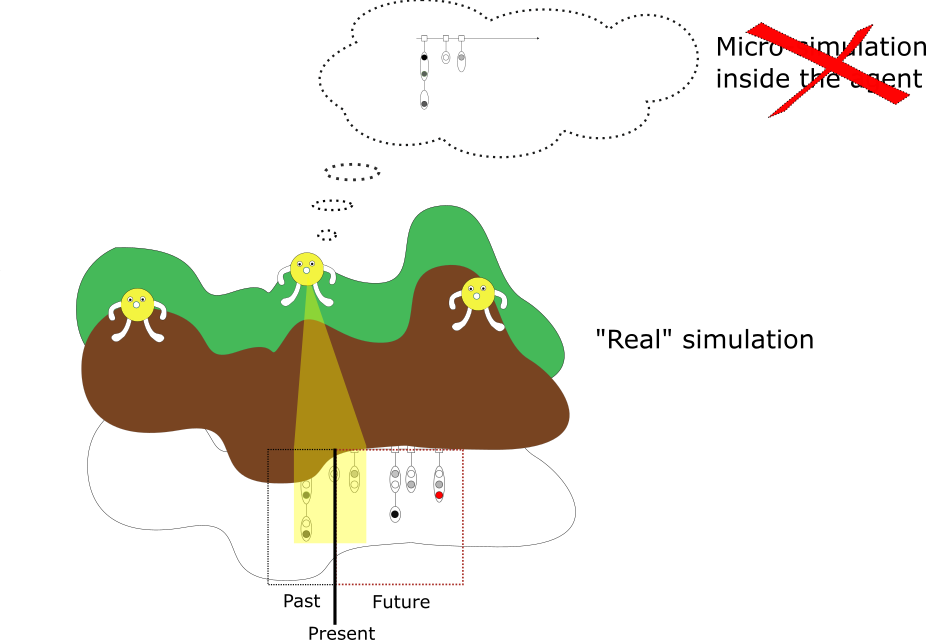
\includegraphics[width=\linewidth]{figures/new_anticipation.png}
    \caption{Anticipatory reasoning using the temporal environment perception}
\end{figure}
\end{column}
}
\end{columns}
\note{
\par Dans la plupart des approches classiques d'anticipation dans les sma, le raisonnement anticipatif prend en compte uniquement les informations sur la dimension passée et la dimension présente du temps. Dans ces types d'approches, l'agent est contraint de deviner ce qui va se passer dans le futur, car ils n'a aucune information sur le planning d'activités des autres agents. Pour se faire, les agents lancent en interne des microsimulations qui génèrent des prédictions. Dans beaucoup d'approches, ces microsimulations reproduisent tout une une partie du modèle de simulation véritablement utilisé.
\par Nous proposons donc une amélioration de ce raisonnement anticipatif par l'intégration de l'environnement temporel qui offre une nouvelle dimension d'expression et de partage entre les agents. La nature temporelle de cette nouvelle dimension permet de capter les projets individuels de chaque agent et de les diffuser sur le collectif. L'analyse prédictive réalisée par les agents peut alors opérer par perception dans ce nouvel environnement commun, plutôt que par des calculs de simulation reproduits par chacun d'eux.
}
\end{frame}

\begin{frame}{A consideration of the future}
\begin{figure}
    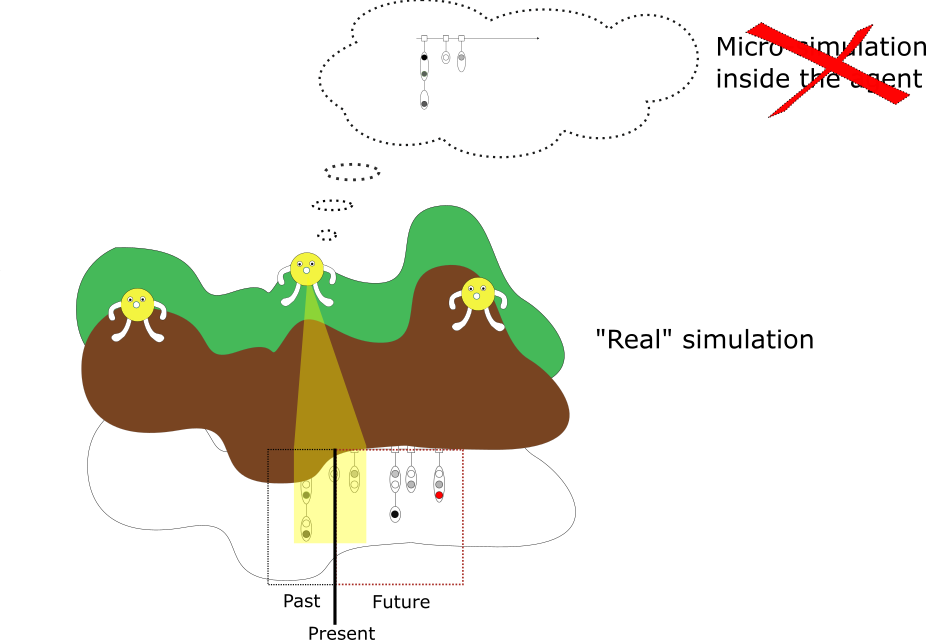
\includegraphics[width=.8\linewidth]{figures/new_anticipation.png}
    \caption{Anticipatory reasoning using the temporal environment perception}
\end{figure}
\note{
\par Nous construisons nos prédiction à partir de la perception des comportements temporels dont l'accès est rendu possible grace à la mise en place de l'environnement temporel. 
\par De plus, contrairement à la plupart des approches classiques qui construisent leur prédisction sur la base des informations passées et présentes, la visibilité sur la dimension future offerte par l'environnement temporel permet à nos agents de prendre en compte les informations temporels positionnées sur le futur.
\par En effet, cette nouvelle dimension d'expression et de partage qui est de nature temporelle permet aux agents de partager leurs projets individuels et de les diffuser sur le collectif. L'analyse prédictive réalisée par les agents se base alors sur la perception de ce nouvel environnement commun, plutôt que par des calculs de simulation reproduits par chacun d'eux.
\par L'état prévisionnel de l'environnement temporel est directement obtenu par perception d'une partie de l'axe temporel contenu dans l'environnement temporel. Cet état prévisionnel est d'autant plus intéressant en ce qui concerne sa précision, car il permet de raisonner sur des informations réelles partagées, au lieu de se baser sur des hypothèses. C'est-à-dire que l'agent n'essaye plus de deviner ce que les autres prévoient de faire comme ce qui est le cas dans la plupart des approches. Dans l'approche que nous proposons, l'agent perçoit les projets individuels des autres agents qui les diffusent sur le collectif, à travers l'environnement temporel.
\par Cela permet à l'agent d'enrichir les informations prises en compte au niveau de son raisonnement anticipatif par des informations sur la dimension future du temps.
}
    
\end{frame}

\begin{frame}{A consideration of the future}{Application}
\par Question agents activity schedule
\par \textbf{Objectives}:
\begin{itemize}
    \item Assess or reassess the feasibility of carrying out an activity
    \item Select the most relevant activity to be carried out
    \item Enrich and bring more precision to the agent's activity planning
\end{itemize}
\begin{figure}
    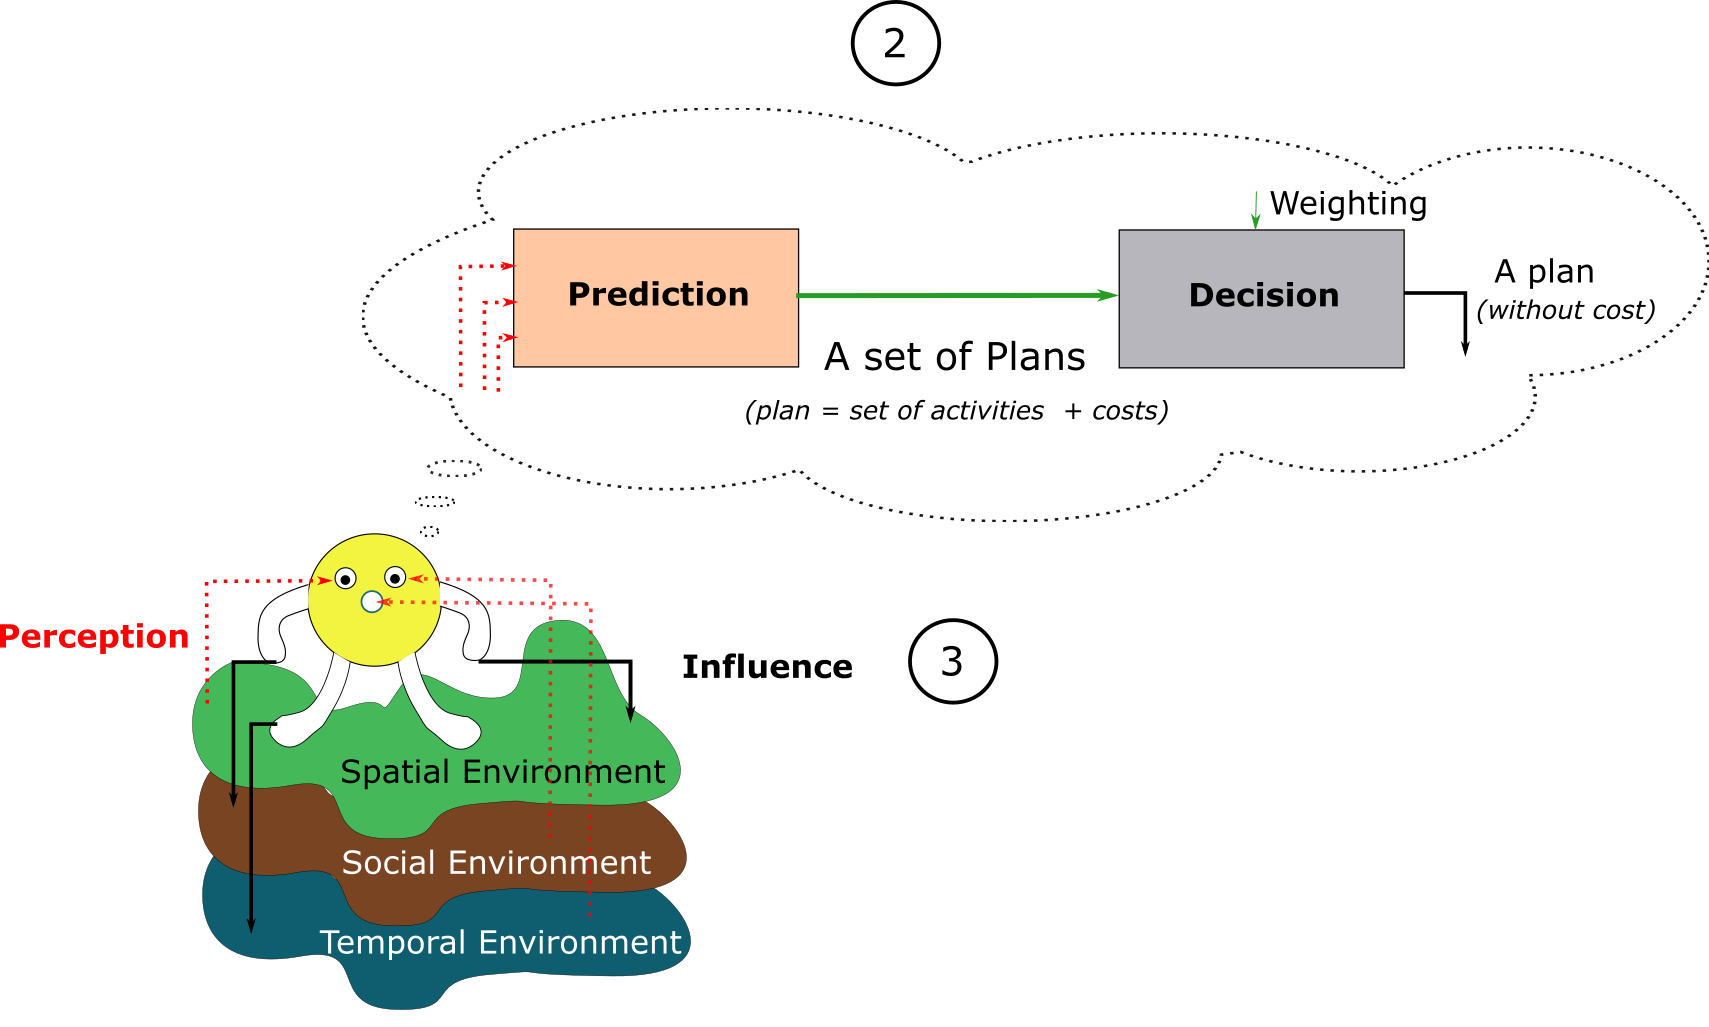
\includegraphics[width=.5\linewidth]{figures/anticipation_cycle.png}
    \caption{Anticipatory reasoning}
\end{figure}
\note{
Dans le raisonnement anticipatif que nous mettons en place au sein des agents du système, nous exploitons les informations que l'agent récolte sous forme de percepts au niveau des différents environnements du système afin de lui permettre de remettre en question son planning d'activités. Les objectifs sont :
\begin{itemize}
    \item évaluer ou réévaluer la possibilité d'exécution d'une activité;
    \item choisir l'activité la plus pertinente à exécuter;
    \item enrichir et apporter plus de précision au planning d'activités de l'agent.
\end{itemize}
\par Le fonctionnement du raisonnement anticipatif consiste en:
\begin{itemize}
    \item L'agent perçoit son contexte d'activation spacial, social et temporel. Plus particulièrement la perception de l'environnement temporel permet de récolter des informations sur le planning d'activité des agents du systèmes, en fonction des horizons temporels (absolues et relatifs) et des règles d'accessibilité. Ce planning contient des informations comportements temporels passées, présentes mais également les projets futurs des agents.
    \item Ces informations sont prises en compte pour générer des prédictions. Ces prédictions prennent la forme d'un ensemble de déclinaison de plan. Ces plans consistement en un enchaînement d'activités avec des coûts. Par exemple: aller travailler à son lieu de travail à 8h avec un cout énergétique de 0.5 sur une échelle de 0 à 1 puis se recharger sur une borne près du lieu de travail avec un coût énergétique de 0 et un coût de longueur prévisionnel de la file de 0.9. ou aller travailler se recharger à 6h sur une borne à proximité du logement du conducteur avec un coût énergétique de 0.1 et un coût en longueur prévisionnel de la file d'attente de 0.1 puis aller travaillet à 8h avec un coût énergétique de 0.5. 
    \item L'agent choisi ensuite le plan le plus pertinent. Pour ce faire, il applique un ensemble de pondération au niveau des coûts. Cela permet de prendre en compte le fait que chaque critère de coût peut avoir une importance différente vis à vis de l'agent et/ou du modélisateur et/ou de l'usager de la simulation. Le choix se base donc sur une minimisation des coûts pondérés. En d'autres termes le plan le plus pertinent est celui donc la somme des coûts pondérée est minimale.
\end{itemize}
}

\end{frame}

\begin{frame}{Temporal reasoning}{Example and implementation}
\begin{columns}
\visible<1->{
\begin{column}{.33\linewidth}
\begin{figure}
    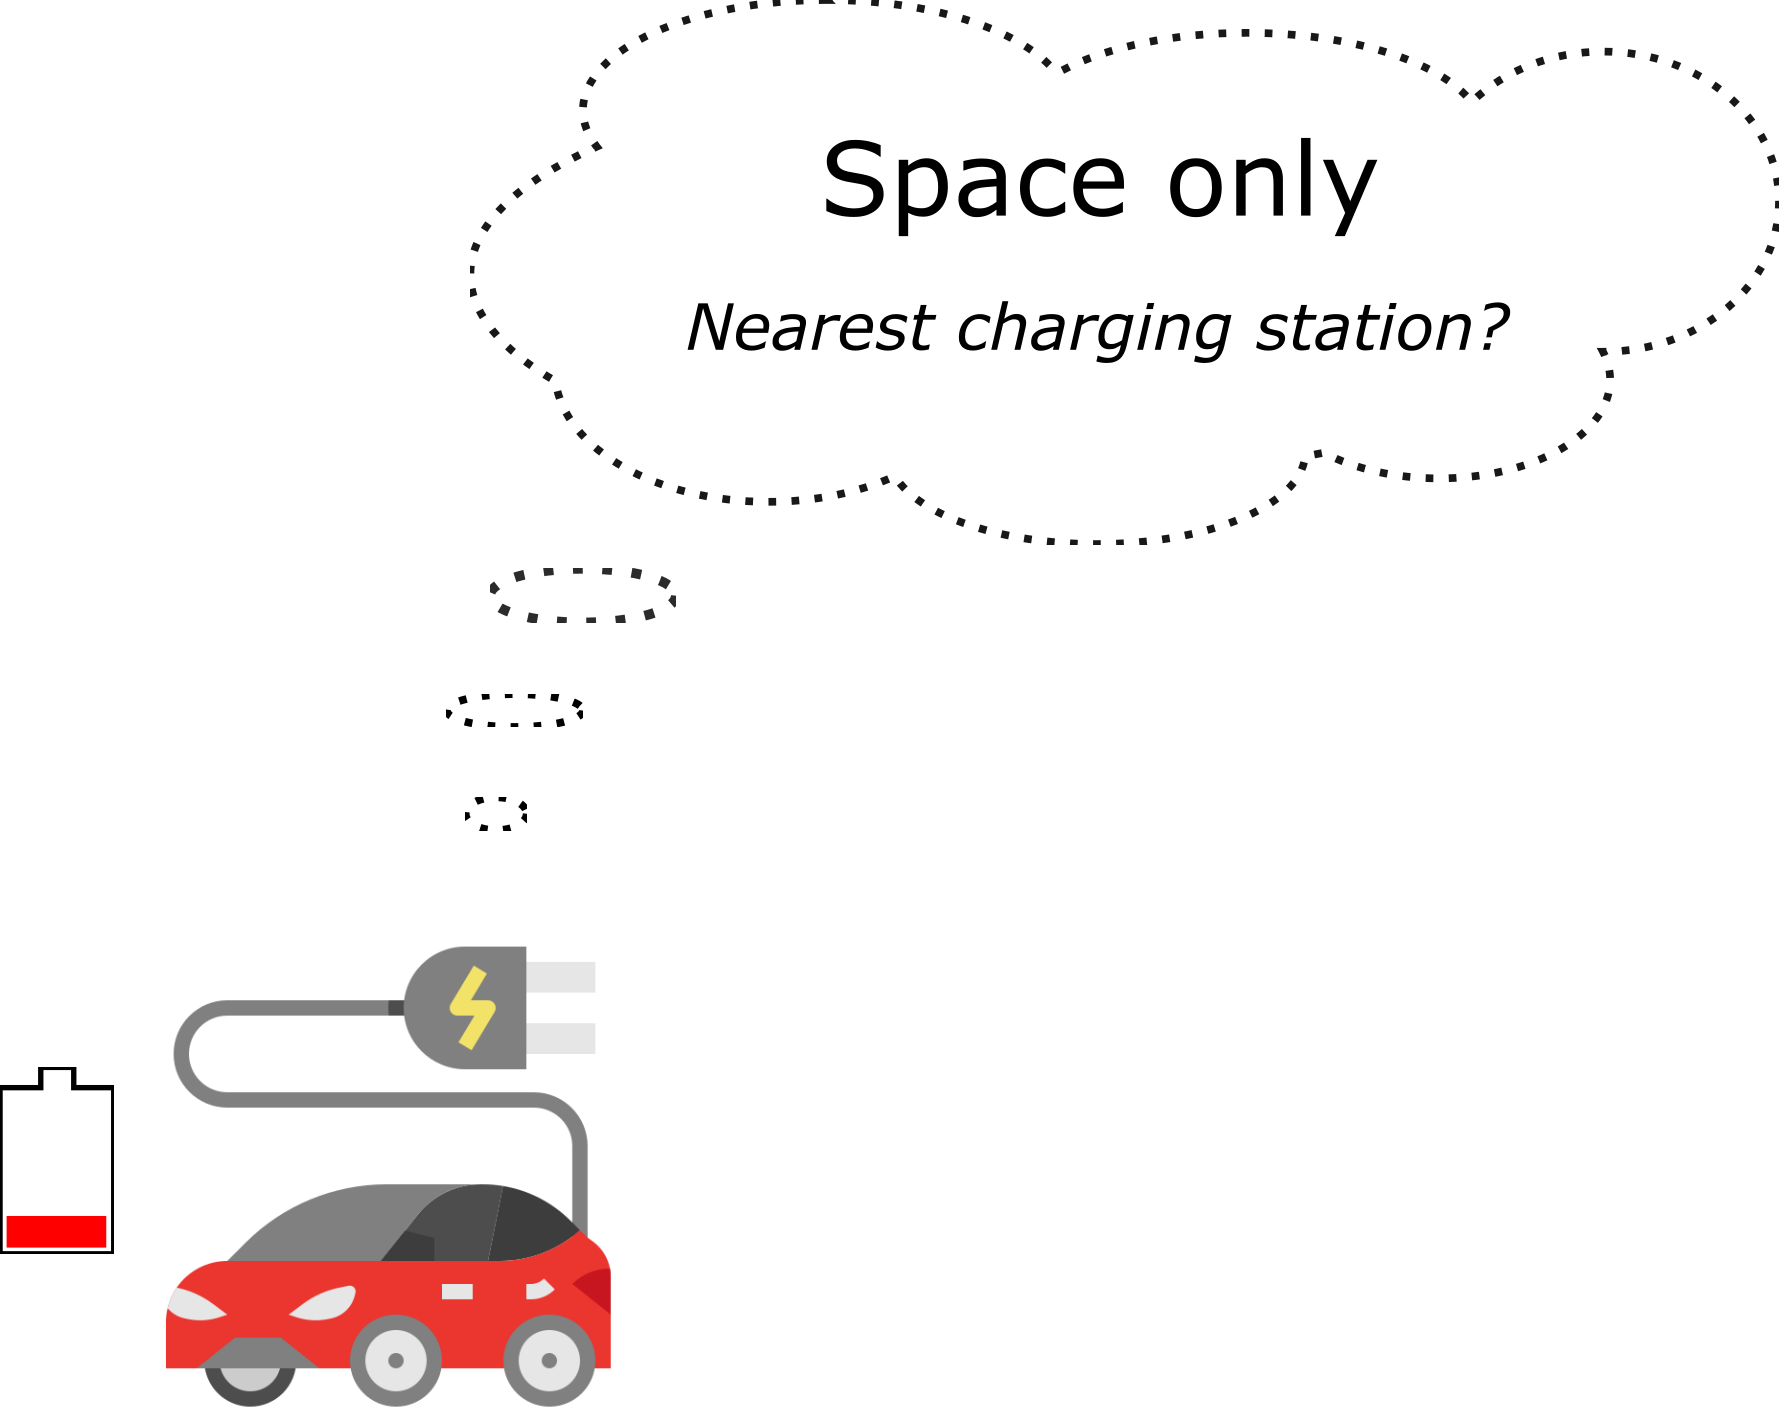
\includegraphics[width=.85\linewidth]{figures/one.png}
   \caption{Classical approach}
\end{figure}
\end{column}
}
\visible<2->{
\begin{column}{.33\linewidth}
\vspace{.3cm}
\begin{figure}
    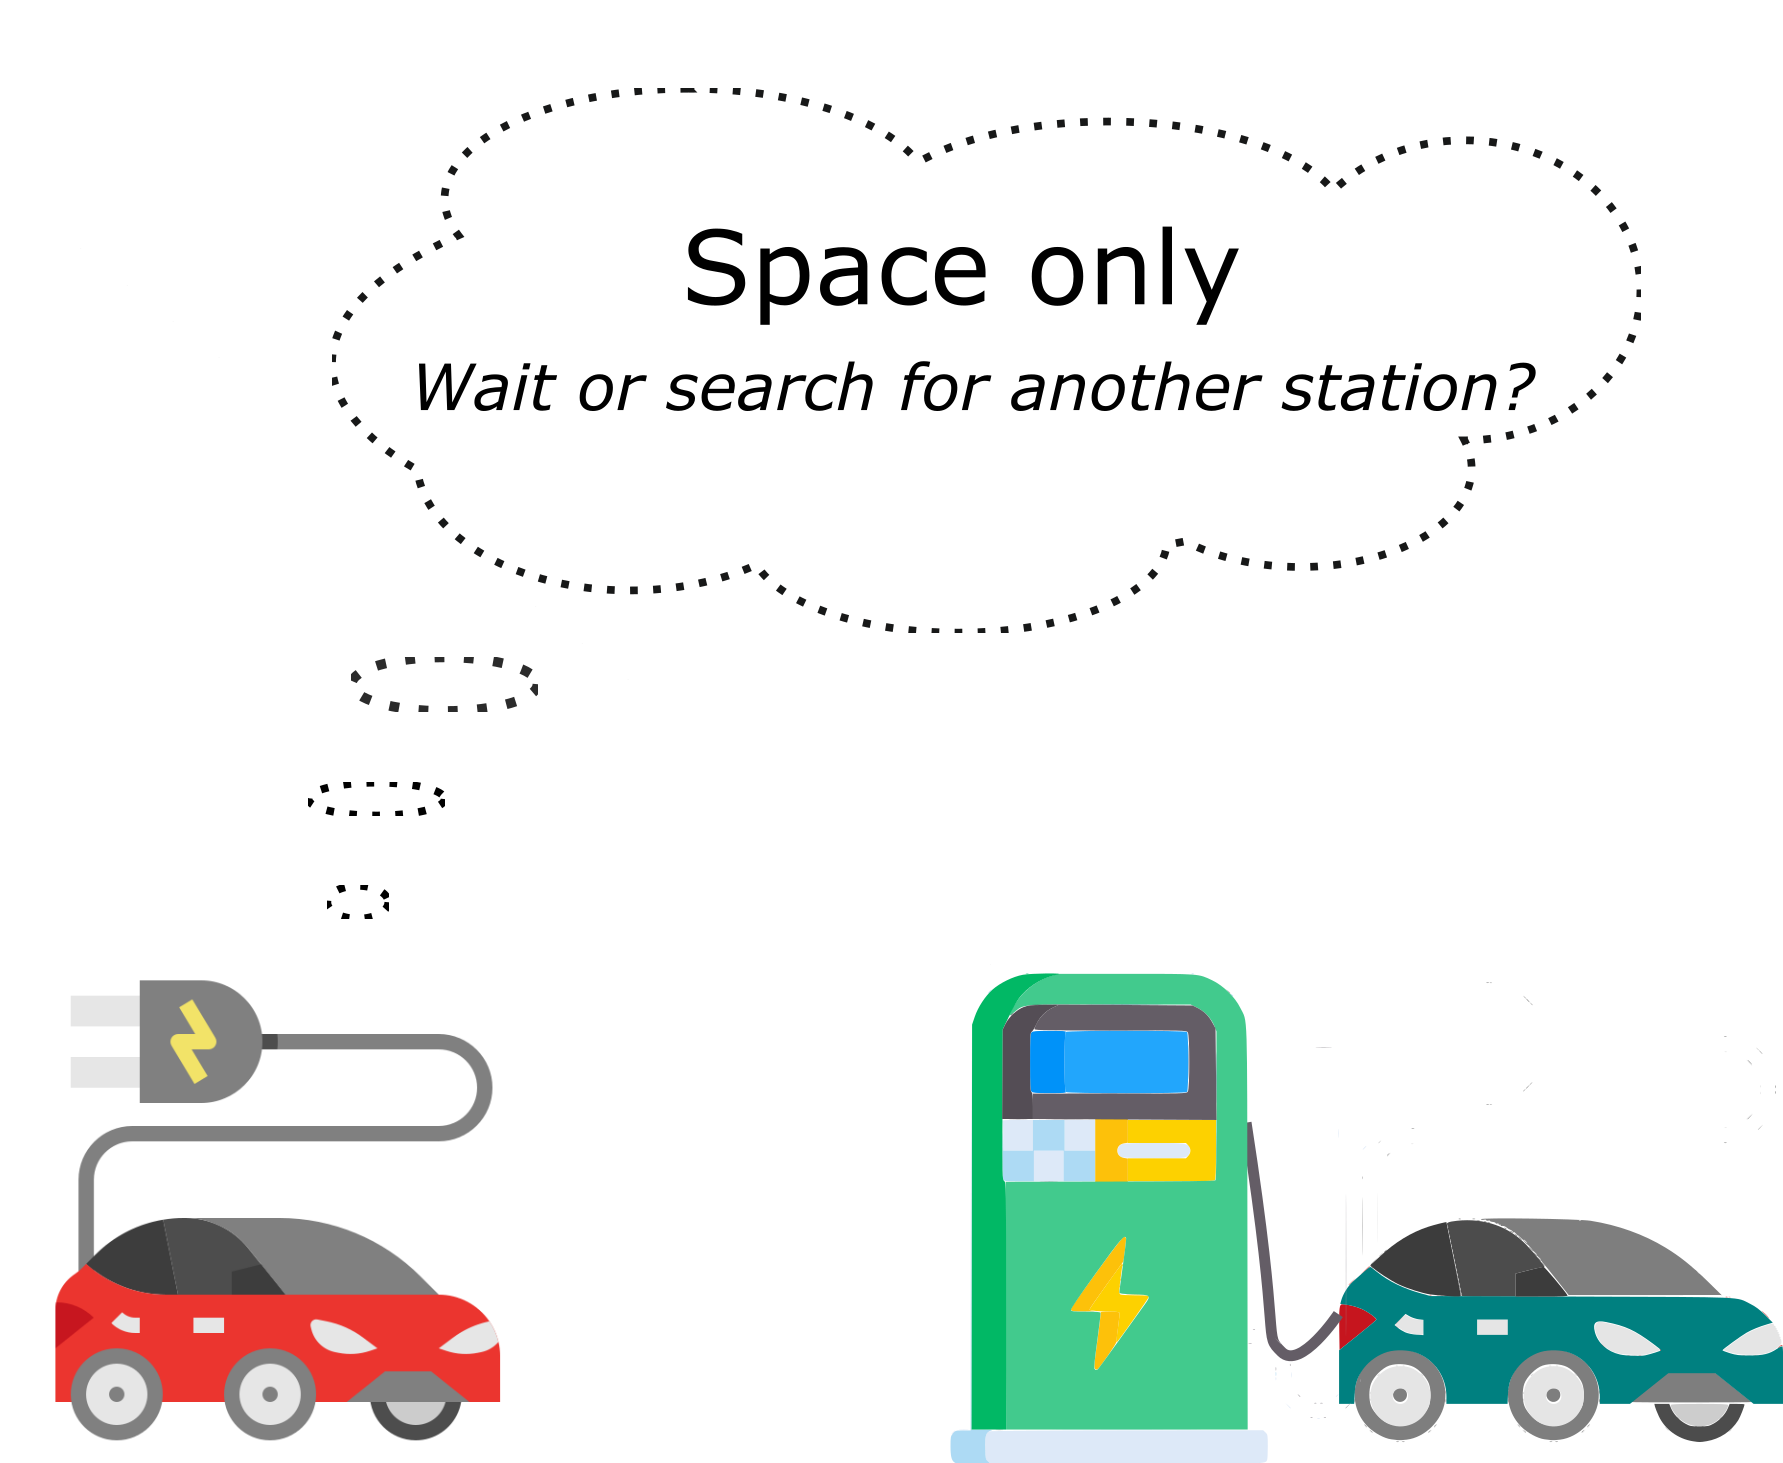
\includegraphics[width=.85\linewidth]{figures/two.png}
\end{figure}
\end{column}
}
\visible<3->{
\begin{column}{.33\linewidth}
\vspace{.4cm}
\begin{figure}
    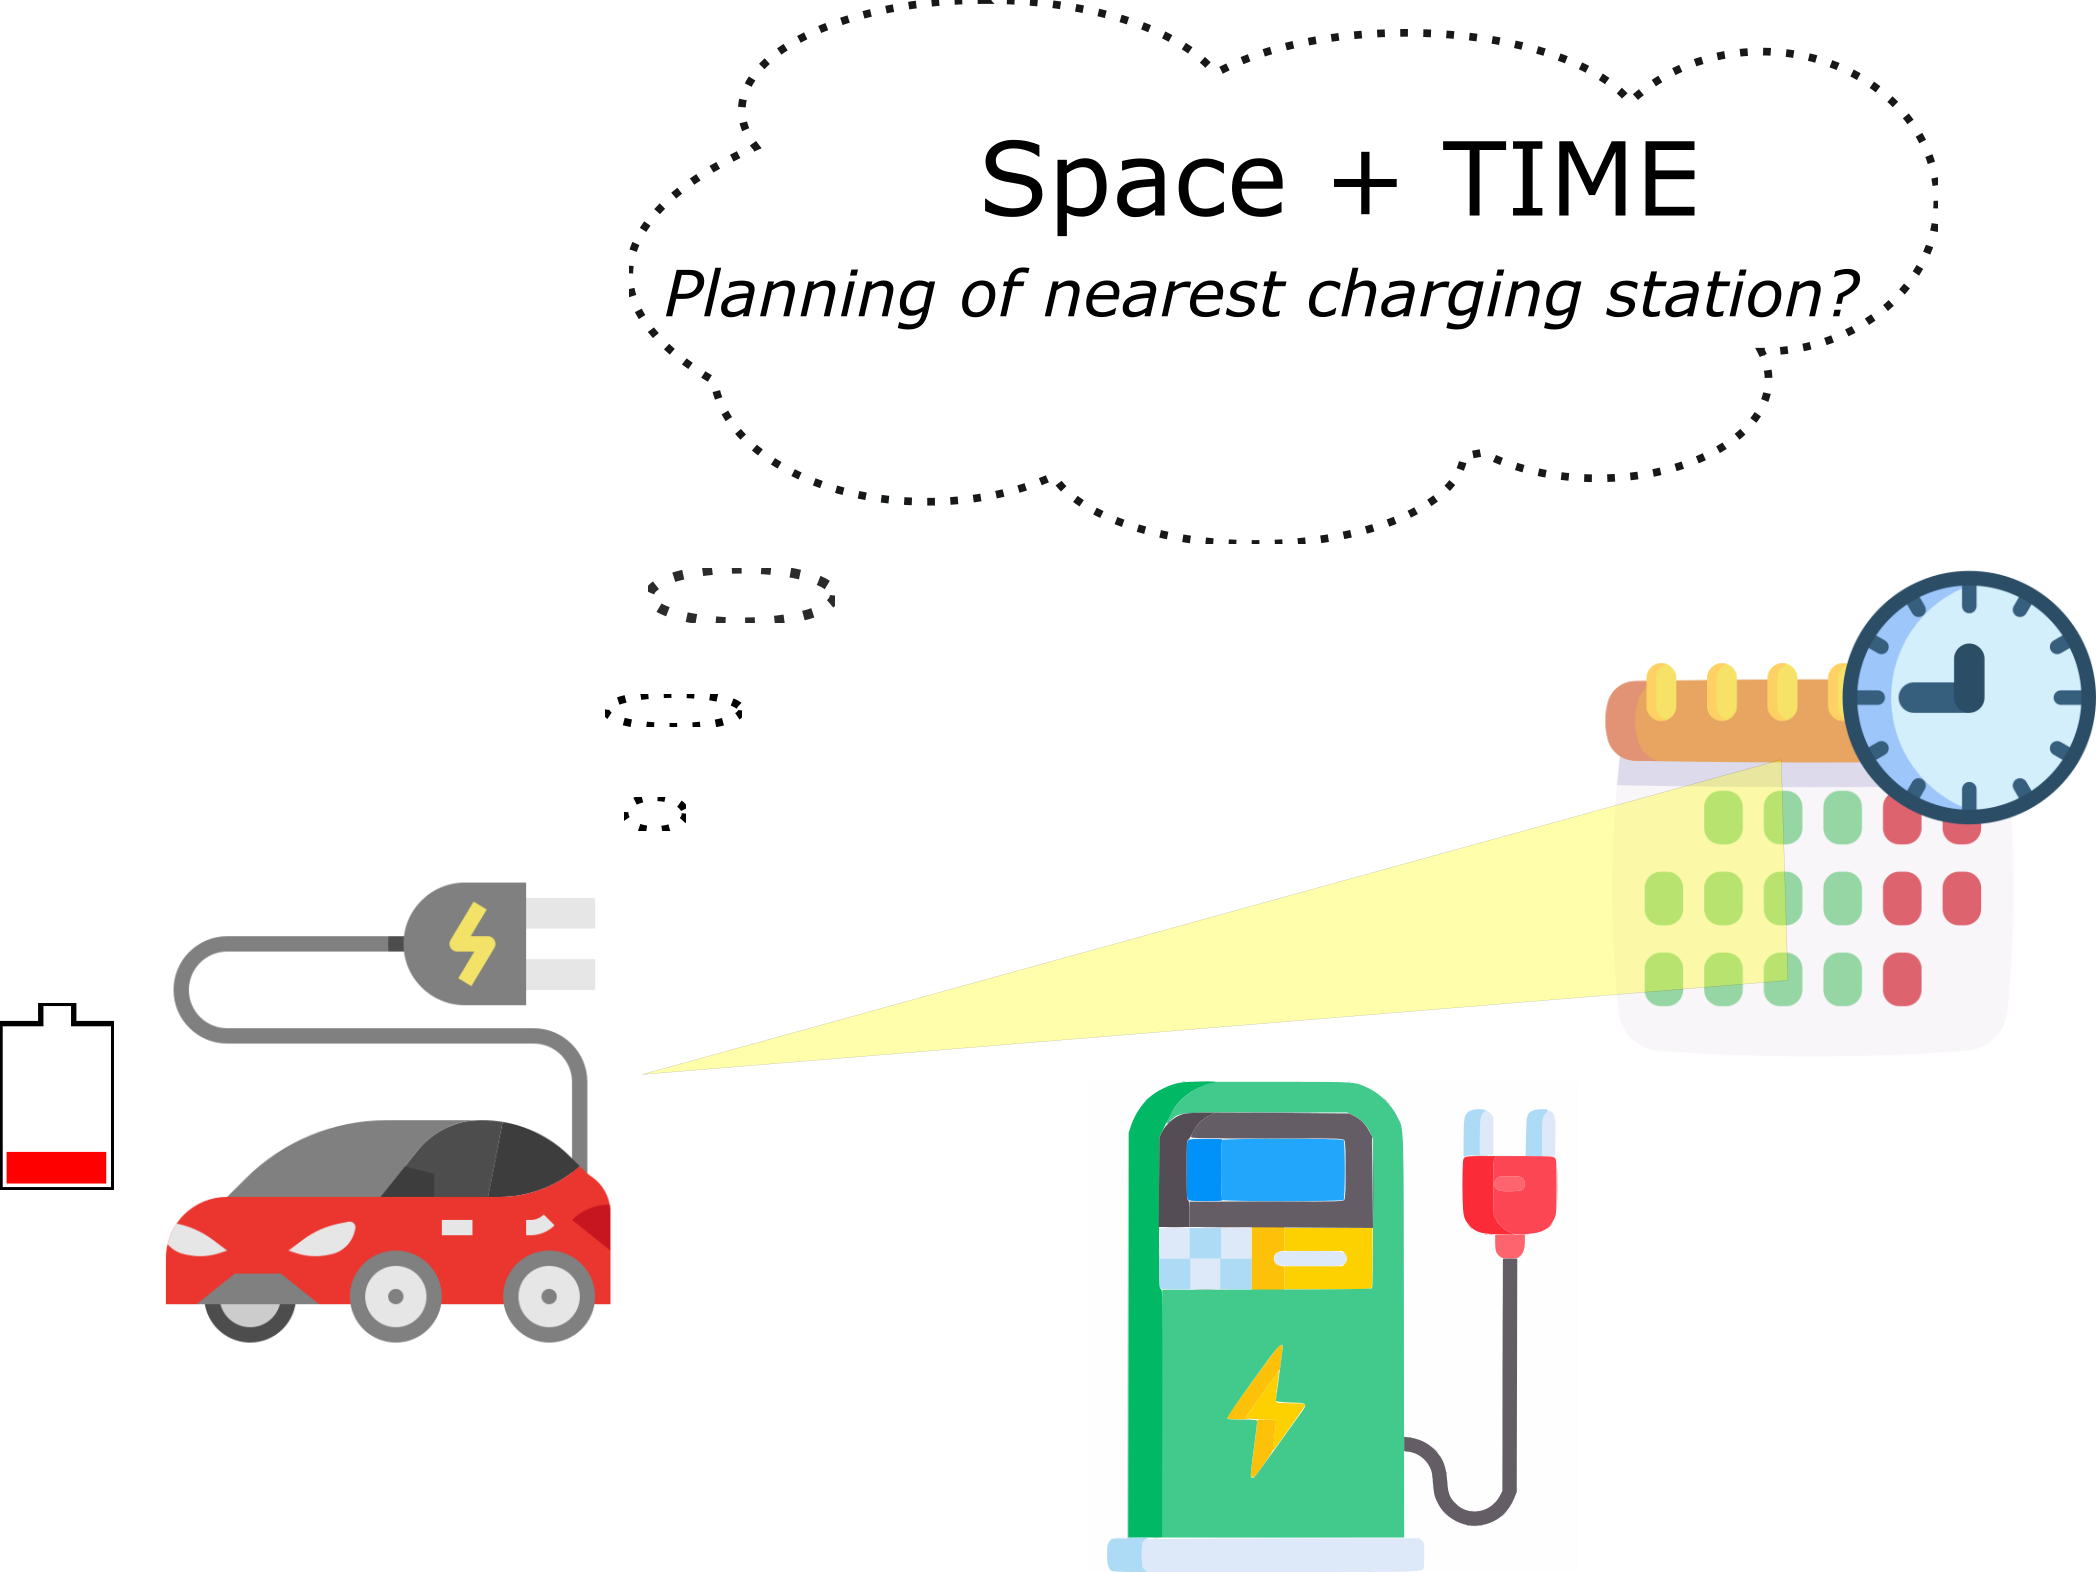
\includegraphics[width=\linewidth]{figures/three.png}
    \caption{Anticipatory reasoning using the temporal environment perception}
\end{figure}
\end{column}
}
\end{columns}


\note{
\par Avant l'intégration de notre contribution, le raisonnement de l'agent se basait uniquement sur le spatial. Par exemple, lorqu'un conducteur de véhicule électrique détecte un niveau de batterie faible de son véhicule, il se met à cherche la borne de recharge la plus proche spatialement et se déplace vers cette borne. Une fois arrivé, si la borne est libre, il s'y branche pour se recharger, sinon il se met dans la file d'attente ou cherche une autre borne libre et répète le processus. 
\par Une autre version un peu plus évoluer de ce système consiste à intéroger les bornes de recharges à proximité spatiales de leur état et de choisir d'aller se recharger vers celle qui est libre. Cependant, rien ne garantit que, le temps d'arriver à cette borne, cette dernière sera encore disponible. Il se peut que d'autres agents aient aussi eu l'idée d'aller s'y recharger et y sont arrivés plus tôt.
\par L'intégration de notre première contribution permet à l'agent d'avoir une visibilité sur le planning d'activité des autres agents du système. Ainsi, le conducteur de véhicule électrique peut avoir une visibilité sur une partie du planning prévisionnel de la borne de recharge. Il peut donc connaître à l'avance si un autre conducteur a prévu de se recharger sur la même borne sur le même créneau. Il aura la visibilité sur la longueur prévisionnelle de la file d'attente. Tout cela lui permet de raisonner sur un espace temporel plus large et de  d'anticiper, avant même d'effectuer le déplacement si sa décision lui semble pertinente vis à vis de ses objectifs ou s'il doit remettre en question une partie de son comportement temporel prévisionnel. 
}
    
\end{frame}